\section{Proposed PHQD Framework}\label{sec:method}

\subsection{System Overview}
PHQD removes Gaussian noise from the latent representation of an image, one small patch at a time, so that each patch fits a few-qubit circuit. Figure~\ref{fig:architecture} shows the workflow. A Fashion-MNIST image is compressed by the encoder of a convolutional autoencoder into a latent map, the map is corrupted with Gaussian noise, and the noisy map is cut into overlapping patches. Each patch is denoised by a hybrid quantum--classical model, the denoised patches are folded back into a latent map by averaging, an optional stitching network refines the result, and the decoder produces the output image. The pipeline is implemented as five modules. Module 1 trains the convolutional autoencoder. Module 2 defines the angle-encoded quantum patch-processing circuit. Module 3 implements a purely classical latent stitching and refinement CNN. Module 4 defines the classical MLP and U-Net baselines. Module 5 implements the EPQD denoisers and the model comparison pipeline.

\begin{figure}[t]
\centering
\IfFileExists{phqd_architecture.png}{
  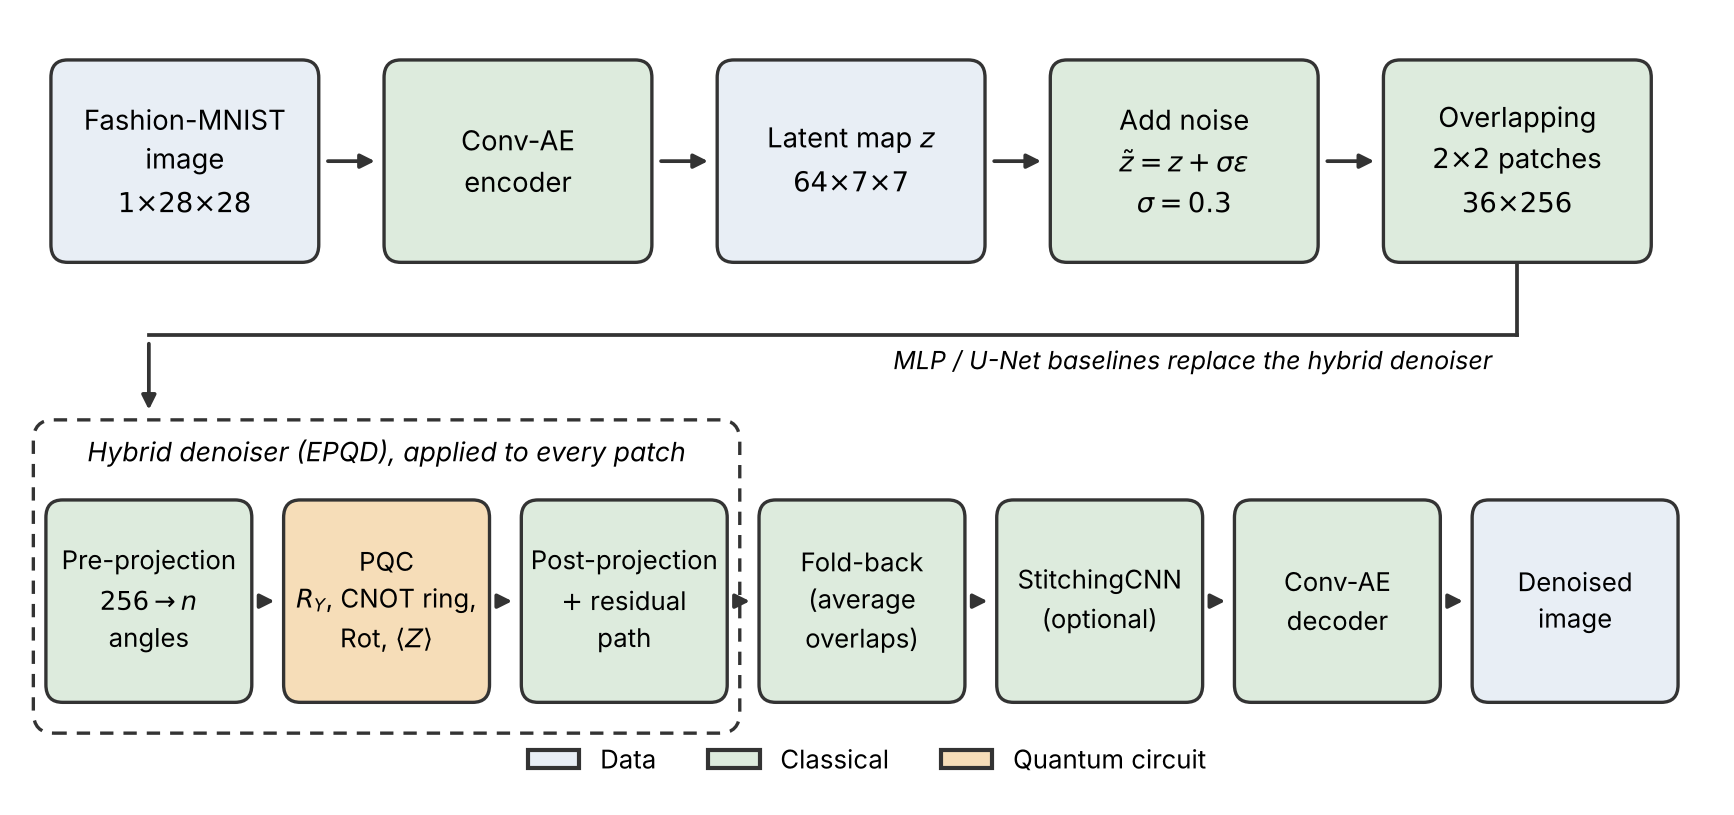
\includegraphics[width=0.98\linewidth]{phqd_architecture.png}
}{
  \fbox{\parbox[c][3.0cm][c]{0.92\linewidth}{\centering Fashion-MNIST image $\rightarrow$ Conv-AE encoder $\rightarrow$ noisy overlapping latent patches $\rightarrow$ EPQD/MLP/U-Net denoising $\rightarrow$ spatial fold-back and optional StitchingCNN $\rightarrow$ Conv-AE decoder.}}
}
\caption{Overall pipeline of the proposed PHQD framework.}
\label{fig:architecture}
\end{figure}

\subsection{Dataset and Preprocessing}
We use Fashion-MNIST~\cite{fmnist}, which contains 60{,}000 training and 10{,}000 test grayscale images of $28\times28$ pixels in ten clothing classes. Images are converted to tensors and normalized with mean 0.5 and standard deviation 0.5, so that pixel values lie in $[-1,1]$. After the autoencoder has been trained and frozen, its encoder serves as the feature extractor and maps every image to a latent map $z\in\mathbb{R}^{64\times7\times7}$ with 3{,}136 values. For denoising, the latent map is corrupted as
\begin{equation}
    \tilde z = z+\sigma\epsilon,\qquad \epsilon\sim\mathcal{N}(0,I),\quad \sigma=0.3.
\end{equation}
A $2\times2$ window with stride one is then slid over the $7\times7$ spatial grid, which gives $6\times6=36$ overlapping patches per image, each flattened to a vector of $64\times2\times2=256$ values.

\subsection{Module 1: Convolutional Autoencoder}
The encoder consists of two strided convolution blocks:
\begin{itemize}
    \item $1\rightarrow32$ channels, $4\times4$ kernel, stride 2, padding 1, followed by batch normalization and LeakyReLU with slope 0.2.
    \item $32\rightarrow64$ channels, $4\times4$ kernel, stride 2, padding 1, followed by batch normalization and LeakyReLU with slope 0.2.
\end{itemize}
This maps $1\times28\times28$ images to $64\times7\times7$ latent tensors. The decoder uses transposed convolutions $64\rightarrow32\rightarrow1$, each with a $4\times4$ kernel, stride 2, and padding 1. Batch normalization and ReLU are used in the first decoder block, and a Tanh output maps the reconstruction to the normalized image range.

The autoencoder is trained with MSE loss and Adam with learning rate $10^{-3}$ for 20 epochs and batch size 128. A cosine annealing learning-rate scheduler is used.

\subsection{Module 2: Quantum Patch Encoding}
For each 256-dimensional patch, the quantum encoder applies a classical projection
\begin{equation}
    a = \tanh\!\left(W_2\,\tanh(\operatorname{LN}(W_1p+b_1))+b_2\right)
    \in[-1,1]^n,
\end{equation}
where $n$ is the number of qubits and LN denotes layer normalization in the first projection block. The output is mapped to rotation angles:
\begin{equation}
    \alpha_i = \frac{\pi}{2}(a_i+1),\qquad \alpha_i\in[0,\pi].
\end{equation}
The circuit applies $R_Y(\alpha_i)$ to each qubit, followed by a ring of CNOT gates and trainable single-qubit rotations. The measured Pauli-$Z$ expectations are then passed through a small classical post-projection.

\subsection{Standard EPQD Denoiser}
The standard EPQD denoiser uses a classical pre-projection from dimension 256 through 128 hidden features to $n$ circuit angles. A Tanh activation bounds the projected values, which are mapped to $[0,\pi]$. For each patch,
\begin{equation}
    a(p)=\frac{\pi}{2}\left(g_{\mathrm{pre}}(p)+1\right).
\end{equation}
The basic PQC first applies $R_Y(a_i)$ on each wire. For each variational layer $\ell$, it applies a cyclic nearest-neighbour CNOT ring and then a trainable \texttt{Rot} gate on each qubit:
\begin{equation}
    U_{\mathrm{basic}}(a,\theta)=
    \prod_{\ell=1}^{L}
    \left[
       \left(\prod_{i=0}^{n-1}\operatorname{Rot}
       (\theta_{\ell i1},\theta_{\ell i2},\theta_{\ell i3})_i\right)
       \left(\prod_{i=0}^{n-1}\operatorname{CNOT}_{i,(i+1)\bmod n}\right)
    \right]
    \left(\prod_{i=0}^{n-1}R_Y(a_i)\right),
\end{equation}
where the written product denotes the implemented ordered gate sequence. The circuit returns
\begin{equation}
    q(p)=\left(\langle Z_0\rangle,\ldots,\langle Z_{n-1}\rangle\right).
\end{equation}
A classical post-projection maps $q(p)$ through dimensions $n\rightarrow128\rightarrow256\rightarrow256$, using LayerNorm and GELU in the first hidden layer and GELU in the next. A learned residual linear mapping is added:
\begin{equation}
    \hat p=g_{\mathrm{post}}(q(p))+W_rp+b_r.
\end{equation}

The PQC is implemented as a batched PennyLane QNode on \texttt{default.qubit}, with \texttt{diff\_method="backprop"}. This uses simulator backpropagation rather than parameter-shift differentiation, and all circuits are therefore simulated classically.

\subsection{IQP-Style Circuit}
The IQP configuration starts with Hadamard gates and data-dependent $R_Z$ rotations on every qubit, followed by nearest-neighbour Ising-$ZZ$ interactions using the product of the first two input angles. Each variational layer then applies the same ring of CNOT gates and trainable \texttt{Rot} gates. The circuit returns Pauli-$Z$ expectation values. This configuration is referred to as EPQD-IQP.

\subsection{EPQD Configurations}
The standard experiment compares the four configurations in Table~\ref{tab:configs}. A separate six-qubit configuration is described later in this section.
\begin{table}[t]
\centering
\caption{Standard EPQD quantum configurations implemented in Module 5.}
\label{tab:configs}
\begin{tabular}{lccc}
\toprule
\textbf{Model} & \textbf{Qubits} & \textbf{Variational layers} & \textbf{Ansatz}\\
\midrule
EPQD-S & 4 & 1 & Basic ring + Rot\\
EPQD-M & 4 & 2 & Basic ring + Rot\\
EPQD-L & 4 & 3 & Basic ring + Rot\\
EPQD-IQP & 4 & 2 & IQP-style + ring + Rot\\
\bottomrule
\end{tabular}
\end{table}

\subsection{Classical Warm-Up and Quantum Fine-Tuning}
Standard EPQD training is conducted in two stages. First, the quantum weights are frozen and a temporary classical linear bypass is used between the pre- and post-projection layers. The classical projection and residual parameters are optimized using the full patch dataset for 10 warm-up epochs, Adam learning rate $10^{-3}$, and cosine annealing. Next, the bypass is removed, the quantum weights are unfrozen, and the full model is fine-tuned for 8 epochs on a randomly selected subset capped at 8{,}000 training patches. The quantum fine-tuning stage uses Adam with learning rate $3\times10^{-3}$ and cosine annealing. Both stages use MSE loss between the denoised and the clean patch, and the batch size is 128.

\subsection{Module 3: Stitching and Latent Refinement CNN}
The StitchingCNN is a classical model that refines a spatial latent map after patch processing. Its stem is a $1\times1$ convolution followed by batch normalization and GELU. It then applies three residual blocks. Each residual block contains two $3\times3$ convolutions with batch normalization, a GELU activation between the convolutions, and a residual addition followed by GELU. A $1\times1$ convolution and Tanh form the head, and a skip mapping is added to the output.

The Module 3 training routine uses frozen autoencoder features, adds Gaussian perturbations with standard deviation 0.15 to latent maps, and trains the StitchingCNN to recover the clean latent map using MSE loss. The default training configuration is 15 epochs, batch size 128, Adam learning rate $10^{-3}$, and cosine annealing. This standalone module is trained without calling a quantum circuit. In the V2 routine, the StitchingCNN is also jointly fine-tuned with EPQD-6Q-V2.

\subsection{Module 4: Classical Baselines}
The MLP baseline operates on flattened 256-dimensional latent patches. Its hidden dimensions are $256\rightarrow512\rightarrow512\rightarrow256\rightarrow256$, using LayerNorm, GELU, and dropout 0.1 after the first two hidden transformations. An identity residual connection adds the input patch to the MLP output.

The U-Net baseline operates on full $64\times7\times7$ latent maps. Its encoder contains two convolutional blocks with channel widths 64 and 128. Each block uses two $3\times3$ convolutions with batch normalization and GELU. Max pooling is used between encoder stages, and a 256-channel bottleneck follows. The decoder uses transposed convolutions and concatenated skip features, followed by convolutional blocks and a $1\times1$ output convolution to restore 64 latent channels.

Both baselines are trained with MSE loss, Adam with learning rate $10^{-3}$, batch size 128, 20 epochs by default, and cosine annealing. The latent noise standard deviation is 0.3.

\subsection{EPQD-6Q-V2: Data Re-Uploading and Multi-Observable Readout}
EPQD-6Q-V2 uses six qubits and three layers. At each layer, it re-uploads the input through $R_Y$ rotations, applies a cyclic CNOT ring, and applies trainable \texttt{Rot} gates. Its quantum readout contains three observables for each qubit:
\begin{equation}
    q_{\mathrm{XYZ}}=
    (\langle X_0\rangle,\ldots,\langle X_5\rangle,
     \langle Y_0\rangle,\ldots,\langle Y_5\rangle,
     \langle Z_0\rangle,\ldots,\langle Z_5\rangle)
    \in\mathbb{R}^{18}.
\end{equation}
The classical post-projection maps 18 features through 128 and 256 hidden units to a 256-dimensional patch vector. A learned residual linear projection is added to the input patch.

V2 training has three phases: (i) 15 epochs of classical warm-up with a temporary bypass and learning rate $10^{-3}$; (ii) 8 epochs of six-qubit circuit fine-tuning with learning rate $2\times10^{-3}$; and (iii) 6 epochs of joint EPQD and StitchingCNN fine-tuning with learning rate $5\times10^{-4}$. The third phase uses at most 60 batches of 16 images per epoch. Its composite objective is
\begin{equation}
\begin{split}
\mathcal{L}_{\mathrm{V2}}={}&
\mathcal{L}_{\mathrm{latent\text{-}MSE}}
+0.5\,\mathcal{L}_{\mathrm{image\text{-}MSE}}\\
&+0.2\left(1-\operatorname{SSIM}(\hat x,x)\right).
\end{split}
\end{equation}
The SSIM term is calculated on images mapped to $[0,1]$, using a $7\times7$ Gaussian window with standard deviation 1.5 and constants $C_1=0.01^2$, $C_2=0.03^2$.

\subsection{Spatial Fold-Back}
Denoised patch vectors are reshaped to their $64\times2\times2$ spatial blocks and placed back at their original latent-grid coordinates. Overlapping estimates are averaged using an element-wise count map:
\begin{equation}
    \hat z(c,h,w)=
    \frac{\sum_{p\in\mathcal{I}(h,w)}\hat p(c,h-h_p,w-w_p)}
         {|\mathcal{I}(h,w)|},
\end{equation}
where $\mathcal{I}(h,w)$ is the set of patches covering spatial location $(h,w)$. The reconstructed latent tensor is passed through the convolutional decoder to obtain the denoised image.

\subsection{Evaluation Metrics}
Reconstruction quality is measured on the Fashion-MNIST test split after decoding and mapping images to $[0,1]$. We report the mean squared error (MSE) and the peak signal-to-noise ratio, $\mathrm{PSNR}=10\log_{10}(1/\mathrm{MSE})$ in dB, between the decoded and the original image, and the structural similarity index (SSIM), which compares local luminance, contrast and structure. Perceptual similarity of whole image sets is measured by the Fr\'echet Inception Distance (FID), computed from Inception-V3 features of 1{,}000 test images. Lower MSE and FID and higher PSNR and SSIM indicate better results.

\subsection{Comparison Setup}
All denoisers receive the same noisy latent maps, generated with $\sigma=0.3$ from the same frozen autoencoder, so that differences in the results come from the denoiser and not from the data. We compare the four 4-qubit EPQD configurations and EPQD-6Q-V2 with the patch-wise MLP and the U-Net of Module 4. The decoded clean latent map (Conv-AE clean) gives the best result that any latent denoiser can reach, and the decoded noisy latent map gives the lower reference. The baselines and the quantum models use the same patch construction, noise level, loss function, optimizer and batch size.
